\documentclass[tikz,border=10pt]{standalone}
\usepackage{newtxtext,newtxmath} % 设置字体为 Times New Roman
\usetikzlibrary{shapes.geometric, arrows.meta, positioning}

\begin{document}
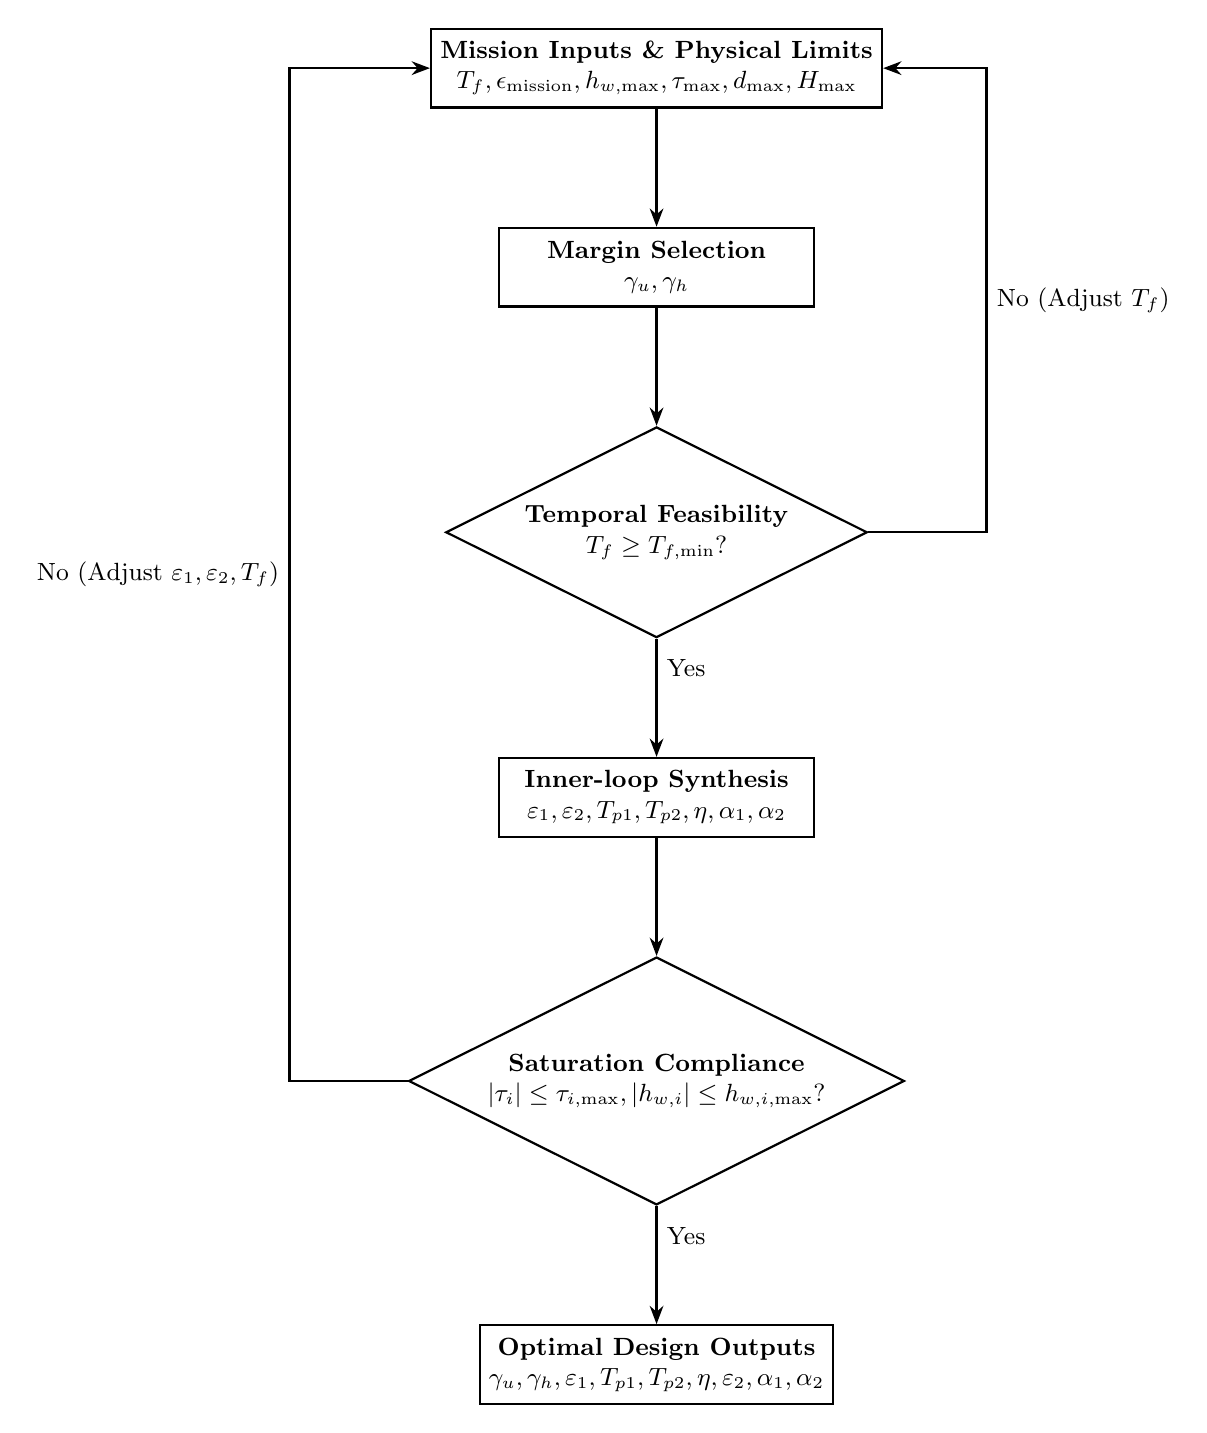
\begin{tikzpicture}[
    node distance=1.5cm,
    every node/.style={font=\small},
    box/.style={rectangle, draw, thick, minimum width=4cm, minimum height=1cm, align=center},
    decision/.style={diamond, draw, thick, aspect=2, minimum width=3.5cm, align=center, inner sep=3pt},
    arrow/.style={-Stealth, thick}
]

% --- 步骤节点 ---
\node (inputs) [box] {
    \textbf{Mission Inputs \& Physical Limits} \\
    $T_f, \epsilon_{\mathrm{mission}}, h_{w,\max}, \tau_{\max}, d_{\max}, H_{\max}$
};

\node (margin) [box, below=of inputs] {
    \textbf{Margin Selection} \\
    $\gamma_u, \gamma_h$
};

\node (check1) [decision, below=of margin] {
    \textbf{Temporal Feasibility} \\
    $T_f \ge T_{f,\min}?$
};

\node (synthesis) [box, below=of check1, node distance=1.8cm] {
    \textbf{Inner-loop Synthesis} \\
    $\varepsilon_1, \varepsilon_2, T_{p1}, T_{p2}, \eta, \alpha_1, \alpha_2$
};

\node (check2) [decision, below=of synthesis, node distance=1.8cm] {
    \textbf{Saturation Compliance} \\
    $|\tau_i| \le \tau_{i,\max}, |h_{w,i}| \le h_{w,i,\max}?$
};

\node (outputs) [box, below=of check2, node distance=1.8cm] {
    \textbf{Optimal Design Outputs} \\
    $\gamma_u, \gamma_h, \varepsilon_1, T_{p1}, T_{p2}, \eta, \varepsilon_2, \alpha_1, \alpha_2$
};

% --- 连接箭头 ---
\draw [arrow] (inputs) -- (margin);
\draw [arrow] (margin) -- (check1);
\draw [arrow] (check1) -- node[right, near start] {Yes} (synthesis);
\draw [arrow] (synthesis) -- (check2);
\draw [arrow] (check2) -- node[right, near start] {Yes} (outputs);

% --- 反馈回路 ---
\draw [arrow] (check1.east) -- ++(1.5,0) |- node[pos=0.25, right] {No (Adjust $T_f$)} (inputs.east);
\draw [arrow] (check2.west) -- ++(-1.5,0) |- node[pos=0.25, left] {No (Adjust $\varepsilon_1, \varepsilon_2, T_f$)} (inputs.west);

\end{tikzpicture}
\end{document}